%%%%%%%%%%%%%%%%%%%%%%%%%%%%%%%%%%%%%%%%%%%%%%%%%%%%%%%%%
%          File: CascadedTunableFilter.tex            	%
%                  Date: 2 Feb, 2015                	%
%                                                    	%
%   For submission to a journal  						%
%                                                     	%
%   Technical paper about the results obtained with   	%
%   professor Wei Shi with tunable cascaded				%
%	contra-directional coupler				      		%
%	+ theorical analysis								%
%%%%%%%%%%%%%%%%%%%%%%%%%%%%%%%%%%%%%%%%%%%%%%%%%%%%%%%%%



\documentclass[9pt,twocolumn,twoside]{osajnl}

\journal{ol} % Choose journal (ao, josaa, josab, ol)

\setboolean{shortarticle}{true}


\usepackage{ulem}
\usepackage{amsmath,amssymb}


\usepackage{graphicx,epsfig,epstopdf}



\title{\underline{Compact} and widely bandwidth-tunable silicon filter with an unlimited free-spectral range}



\author[1]{Jonathan St-Yves}
\author[1]{Hadi Bahrami}
\author[1]{Philippe Jean}
\author[1]{Sophie Larochelle}
\author[1,*]{Wei Shi}
\affil[1]{Centre d'optique, photonique et laser (COPL) and Département de génie électrique et génie informatique, Université Laval, 2375 rue de la Terrasse, Québec (Québec), Canada, G1V 0A6}
\affil[*]{Corresponding author: wei.shi@gel.ulaval.ca}

\dates{Compiled \today}

\ociscodes{ (130.7408) Wavelength filtering devices; (350.2770) Gratings; (130.3120)   Integrated optics devices}

\doi{\url{http://dx.doi.org/10.1364/ao.XX.XXXXXX}}

\begin{abstract}
	Next-generation high-capacity optical networks require flexible allocation of spectrum resources, for which low-cost optical filters with an ultrawide bandwidth tunability beyond hundred GHz are desired.
	We demonstrate an integrated band-pass filter with the bandwidth continuously tuned across 670 GHz (117 GHz to 788 GHz), which, to the best of our knowledge, is the widest tuning span ever demonstrated on a silicon chip.
	The filter also features simultaneous wavelength tuning and an unlimited free spectral range. 
	We measured an out-of-band contrast of up to 55 dB, low in-band ripples of less than 0.3 dB, and in-band group delay variation of less than 8 ps.
	This result was achieved using cascaded Bragg-grating-assisted contra-directional couplers and micro-heaters on the 220-nm silicon-on-insulator platform with a footprint of less than \underline{7,000~\textmu m$^2$.} Another design with the bandwidth continuously tunable from 50 GHz to 1 THz is also presented. 
\end{abstract}

\setboolean{displaycopyright}{true}

\begin{document}
	\maketitle
	\thispagestyle{fancy}
	\ifthenelse{\boolean{shortarticle}}{\abscontent}{}
	
	%\section{Introduction}
	
	Next-generation optical transmission systems applying flexible networking and the super-channel technique will require highly dynamic channel allocation to drastically increase the spectral efficiency and transmission capacity \cite{jinno2009spectrum, geisler2011demonstration}.
	Tunable optical filters, reconfigurable in both center wavelength and bandwidth with scalability towards terahertz \cite{geisler2011demonstration}, are essential for these applications.
	Such large bandwidth tunability is currently only available in bulky bench-top systems using diffractive grating spectrometers or liquid crystals.
	Integrated solutions are desired for lower cost and power consumption.
	In particular, silicon photonics  based on the sub-micron silicon-on-insulator platform allows for CMOS compatible mass fabrication, enabling low cost, high yield, and high-density chip-scale integration.
	Existing solutions for tunable  filters on silicon include devices based on microring resonators \cite{DynamicBW, ong2013ultra} and Mach-Zehnder interferometers (MZIs). These devices have relatively small tunable bandwidth (less than 200 GHz) and small free spectral range (FSR) -- typically less than 10 nm, unable to cover the entire C-band, which are not suitable for high-capacity transmission applications.
	
	Contra-directional couplers(contra-DCs) are grating-assisted add-drop filters \cite{shi2013siliconContraDC}. 
	Analogous to waveguide Bragg gratings, the wavelength selectivity in contra-DCs is based on periodic dielectric perturbations. But instead of back-reflections in the same waveguide, the selected wavelength in a contra-DC is dropped to another waveguide through contra-directional coupling.
	This allows add-drop operation without the need of a circulator. 
	Contra-DCs have merits of compactness, flat-top response, flexible filter design (e.g, through apodization), and near-infinite FSR (in the case of first-order gratings).
	In particular, they allow for very high bandwidths (greater than 10 nm) and thus can support very-high-baud-rate super-channel signals \cite{jinno2009spectrum}.
	In this paper, we demonstrate a broadband filter with a large tunability in both wavelength and channel bandwidth, using thermally controlled cascaded contra-DCs on a silicon chip. 
	The filter has flat-top responses, low insertion loss, low in-band ripples, and high contrast between the pass-band and the stop-band.
	
	\begin{figure}[htbp]
		\centering
		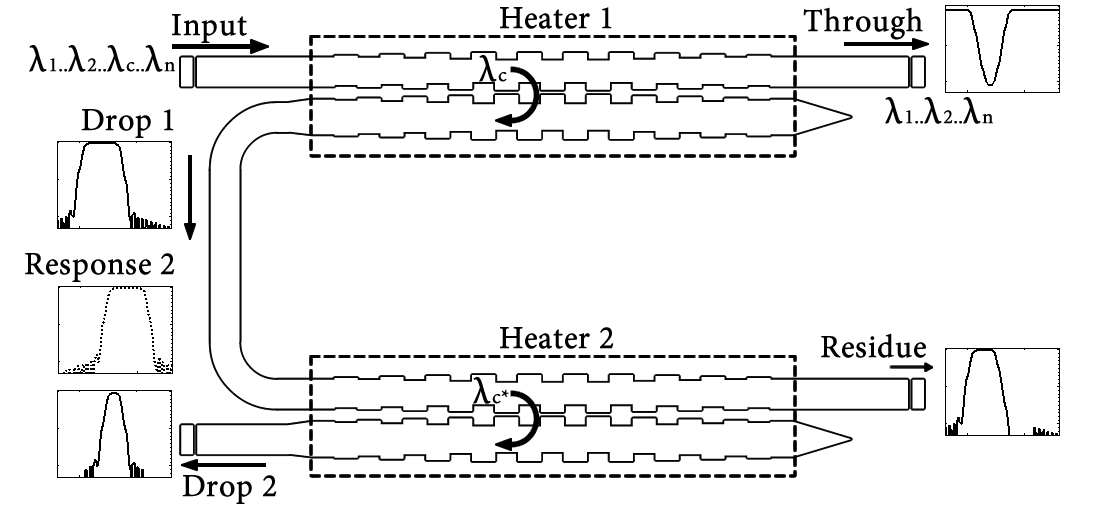
\includegraphics[width=1.00\columnwidth]{data/CascadedSchematic2}
		\centering
		\caption{Schematic of the device. 
			The dropped wavelength of the first contra-directional coupler is re-filtered in an identical component. 
			Both contra-directional couplers are temperature-controlled with metal heaters. 
			Plots show examples of spectrum at each port, on a logarithmic scale.}
		\label{fig:schematic}
	\end{figure}
	%\section{Principle and Design}
	
	The schematic of the proposed device is shown in Fig.~\ref{fig:schematic}. 
	It consists of a pair of cascaded contra-DCs, each operating as a drop filter. 
	The drop port of the first contra-DC is connected to the input port of the second contra-DC. 
	Therefore, the finally dropped signal ("Drop port of the system"), is determined by the product of the  drop-port transfer functions of the two contra-DCs. 
	
	\sout{The center wavelength of the contra-DC is determined by the phase-match condition: $\lambda_\text{c} = \Lambda (n_\text{1}+n_\text{2})$, where $\Lambda$ is the grating pitch, and $n_\text{1}$ and $n_\text{2}$ are the effective indices of the first-order and second-order eigenmodes in the coupler.}
	At first, the two filters are identical and drop a large, well-defined window. By changing the temperature of a single filter, the bandwidth of the finally dropped signal can be adjusted by detuning the center wavelengths of the two contra-DCs.
	
	
	
	\begin{figure}[htbp]
		\centering
		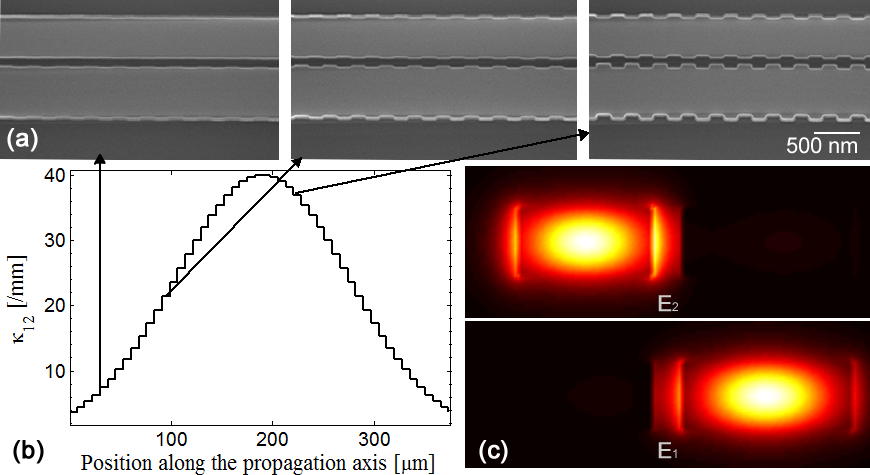
\includegraphics[width=1\columnwidth]{data/FigApod}
		\caption{(a)SEM photography of a part of the grating. The contra-directional coupler consists of two close waveguides of different width with periodic sidewall corrugations. (b) Apodization profile of the grating. A larger coupling requires larger corrugations. (c) Intensity distributions of electrical fields of the first and second transverse modes. }
		\label{fig:SEM}
	\end{figure} 
	
	
	A broadband filter design for a coarse WDM on the 220-nm SOI platform \cite{shi2013siliconCWDM} is adopted for individual contra-DCs.  
	In each contra-DC, the widths of the waveguides are 560 nm and 440 nm.
	This high asymmetry ensures a negligible forward cross-coupling. 
	The gratings are formed by sidewall corrugations in strip waveguides with a pitch of 312 nm.
	Each contra-DC has 1,000 grating elements for a length of 312 \textmu m.
	The spacing between the waveguides varies between 65 and 135 nm to produce a Gaussian-profiled coupling apodization as shown in Fig.~\ref{fig:SEM} for efficient sidelobe suppression, for which details can be found in \cite{shi2013siliconCWDM}.
	
	The spectral responses of each contra-DC is calculated using coupled mode theory and the transfer matrix method, following the same procedure as in  \cite{shi2013siliconContraDC}, with three additions: apodization, temperature dependence and noise simulation.
	While an unapodized (uniform) grating can be simulated with only two transfer matrices,
	an apodized design needs an independent matrix for each grating element along the propagation, to match the change of coupling, and the transfer matrix of the entire contra-DC is given by the product of all the grating elements along the propagation axis.
	Our simulations use 100 segments to approximate the continuously varied coupling.
	
	On top of each contra-DC sits a metal strip acting as a micro-heater for thermal tuning.  
	The refractive index of silicon has a temperature dependence of 
	${\mathrm{d}{n_\text{Si}}}/{\mathrm{d}T}=$ 1.87$\times10^{-4}$K$^{-1}$
	at room temperature for wavelengths around 1550 nm~\cite{frey2006temperature}.
	Without electrical input, the optical responses of the two filters are in principle identical (except for fabrication errors), resulting in a sharp transition from the pass-band to the stop-band. 
	Applying independent electrical currents on the heaters, we can shift the spectra of the contra-DCs simultaneously or differentially for wavelength or bandwidth tuning.
	Ideally, each contra-DC should be uniformly heated so that the apodization profile would not be disturbed as the temperature varies.
	In simulation, the temperature dependence is accounted for by 
	$\mathrm{d}n_\text{eff}=\mathrm{d}n_\text{Si}/{\mathrm{d}T}\times\mathrm{d}n_\text{eff}/{\mathrm{d}n_\text{Si}}\times\mathrm{d}T$, where $\mathrm{d}n_\text{eff}/{\mathrm{d}n_\text{Si}}$ is evaluated using an eigenmode solver.
	
	While only coupling apodization has been discussed so far, it is common in Bragg grating profiles to also adjust the local Bragg wavelength. This can be done with a phase shift changing the local effective index or period. This design only uses coupling apodization in principle, but phase noise also appears during fabrication due to non-uniformity and sidewall roughness.
	
	There are two main types of waveguide noise considered in our simulation. High-frequency phase noise (typically around 10 \textmu m of spacial period \cite{simard2013characterization}) is caused by sidewall roughness and decreases the sidelobe suppression. Low-frequency phase noise, with a correlation length larger than the device (300 \textmu m), is caused by the wafer thickness non-uniformity and etching variance, resulting in a linear chirp that increases the bandwidth.
	High frequency phase noise is considered in our simulation by adding random noise $\Delta\hat{\beta}$ to the propagation constants. The frequency distribution of the noise thus matches the quantization steps of the matrices, but since the response noise is dependent on both the amplitude and frequency of the sidewall roughness \cite{simard2011impact}, we can fit the simulation to the experiment by choosing the right noise amplitude.
	Similarly, we can also add a variation to $\Delta\hat{\beta}$ which is dependent on the longitudinal position.
	
	
	%\section{Experiment}
	
	The device was fabricated using a CMOS-compatible technology with electron-beam lithography. 
	\uline{Large coupling coefficients and precise apodization profiles are easier to achieve with this process, although optical lithography able to create the required periodicity and gap between waveguides as seen in \ref{fig:SEM} a) could be used. The corrugations do not need to be square shaped, but must have a large enough amplitude.}
	
	Fiber grating couplers \cite{zhong2014focusingFGC} are used as optical inputs and outputs in the measurement. 
	Fig.~\ref{fig:passive} shows the measured drop port response of the cascaded contra-DC filters. 
	The measurements were normalized using the response of a pair of directly connected fiber grating couplers on the same chip.
	\begin{figure}[htbp]
		\centering
		\includegraphics[width=.99\columnwidth]{data/Passive62}
		\caption{ Spectral response of the cascaded filters without heating: 1-dB BW is 733 GHz, 3-dB BW is 788 GHz, 10-dB BW is 868 GHz, and 20-dB BW is 990 GHz. Inset shows the filter shape up to -20 dB, which is the typical communication requirement.}
		\label{fig:passive}
	\end{figure}
	
	The device exhibits a high side-lobe suppression ratio (SLSR) of over 40 dB and a high contrast of about 55 dB between the pass-band and the stop-band. 
	The insertion loss is very low, less than 0.5 dB (i.e., 0.25 dB per contra-DC), with small ripples of less than 0.3 dB within the 1-dB passband over 5.8 nm (733~GHz). \uline{This agrees with the measurements in the literature \cite{caverley2015measurement}.}
	The edge roll-off rate is 19 dB/nm on the left side and 24 dB/nm on the right side.
	The simulation agrees well with experiment.
	
	%\subsection{Phase}
	\begin{figure}[tbp]
		\centering
		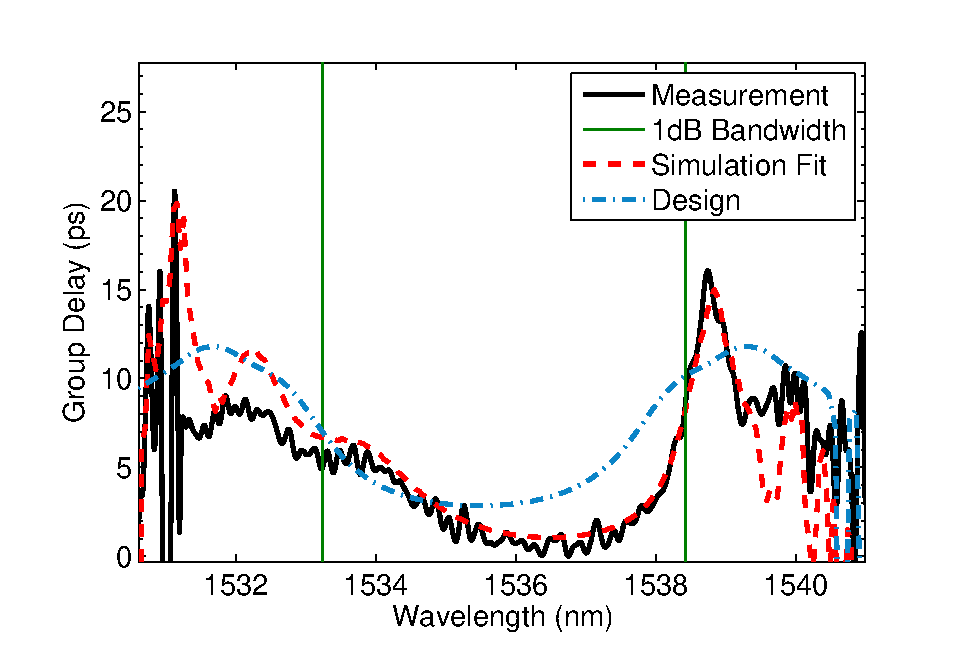
\includegraphics[width=.99\columnwidth]{data/Phase3}
		\caption{ Group delay response of the tunable filter at the drop port. The delay stays within 8 ps between any two points in the band. The out of band results are noisy due to the weak signal.}
		\label{fig:phase}
	\end{figure}
	Another important parameter to monitor is the group delay, as an uneven delay within the pass band may cause signal distortion. The simulation and measurements seen in Fig.~\ref{fig:phase} both show a group delay difference of less than 8~ps within the 1-dB bandwidth. 
	Compared to the original design without considering the phase noise due to fabrication errors, the measured group delay shows a slight distortion. Good agreement is obtained by taking into consideration the linear chirp caused by the silicon wafer thickness variation.
	
	Further work could optimize the grating structure further using the inverse layer peeling algorithm\cite{skaar2001synthesis} since the mathematics of the contra-directional coupler are similar to those of Bragg gratings.
	
	By changing the temperature of a single contra-DC, we shift its phase-match condition, resulting in a smaller band overlap between the two contra-DCs and thus a narrower passband in the drop port, as shown in Fig.~\ref{fig:bandTune}.  
	Due to the wavelength detuning,  the stop-band edges are now determined by the single filters. 
	\uline{As a result, the side-lobes suppression for small bandwidths degrades to -15 dB.}
	A continuous tuning of the 3-dB bandwidth from 788 GHz down to 117 GHz (i.e., over 670 GHz or 5.4 nm) is experimentally observed as the on-chip temperature increases by 70 degrees. 
	
	The microheaters are made of 300-nm-thick, 2-\textmu m-wide Al strips.
	\uline{The power efficiency of the bandwidth tuning is about 24~mW/nm, which dissipates a lot of heat and would be impractical for integration with electronics.}
	We also observe a slight red-shift of the center wavelength at higher temperature, indicating thermal coupling between the two contra-DCs that are about 10 \textmu m away from each other.
	\uline{These issues can be resolved by optimizing the heater design, e.g., using smaller heater features and thermal isolation \cite{dong2010thermally}.}
	
	
	
	\begin{figure}[htbp]
		\centering
		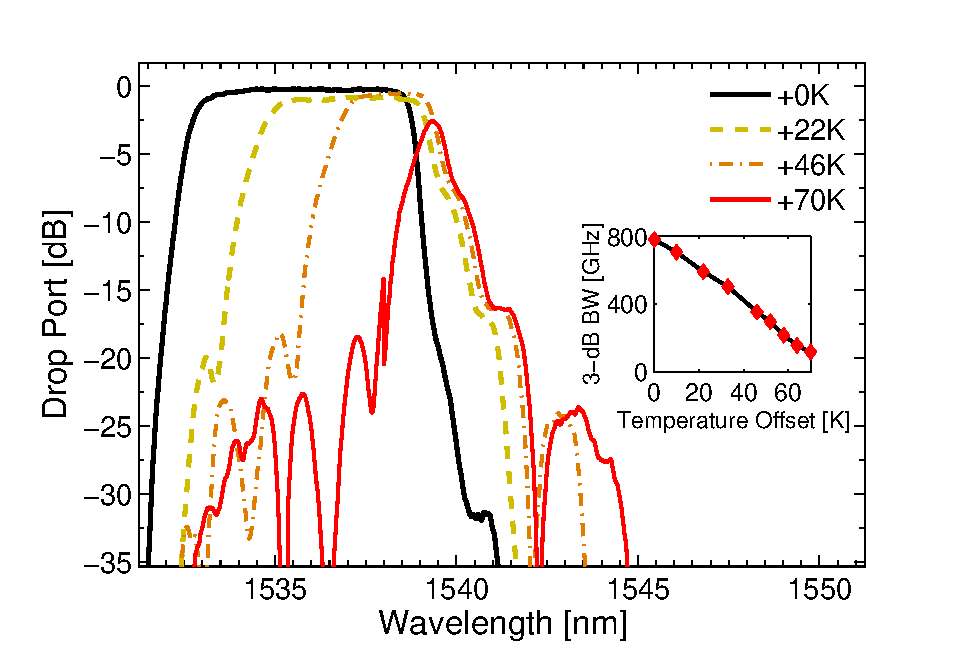
\includegraphics[width=.99\columnwidth]{data/Band6}
		\caption{Spectral response of the device for different temperatures applied to only one contra-DC: 1-dB BW tuned down to 65 GHz, 3-dB BW to 117 GHz. The temperatures are obtained from simulation fit. Inset shows the temperature dependence.}
		\label{fig:bandTune}
	\end{figure} 
	
	By applying the same temperature variation on both contra-DCs, the center wavelength can be tuned without affecting the filter shape.
	As shown in Fig.~\ref{fig:wavTune}, when the center wavelength is continually changed over 4 nm by varying the on-chip temperature, the filter shape is maintained with sharp edges. 
	%Actually, slight detuning between the cascaded contra-DCs may be used to compensate for band-edge distortions due to fabrication errors for a more symmetric filter shape. 
	The power efficiency of the wavelength tuning is about 44~mW/nm, which is about twice the power consumption of the bandwidth tuning since two contra-DCs are heated simultaneously.
	\begin{figure}[htbp]
		\centering
		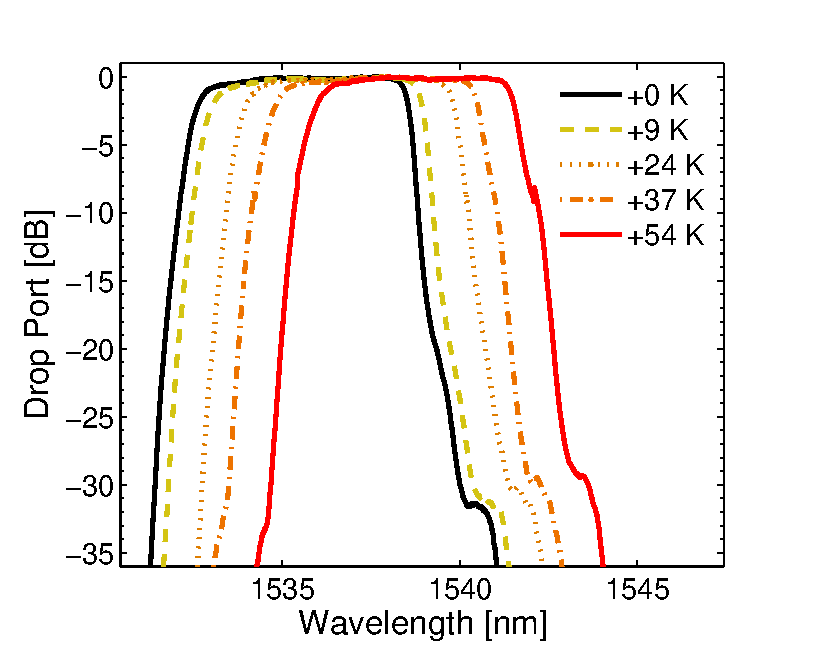
\includegraphics[width=.99\columnwidth]{data/Central2}
		\caption{Spectral response with the heat applied to both contra-DCs: the central wavelength is tuned from 1535 nm to 1539 nm continuously; the temperatures are calculated by comparison to simulation. Inset shows the temperature dependence.}
		\label{fig:wavTune}
	\end{figure} 
	
	
	
	
	
	
	
	\begin{table*}[thb]
		\caption{Recent results with multi-element on-chip silicon filters}
		\begin{tabular}{cccccc}
			\hline
			Publication & Filter type & BWmax / FSR & Tunable BW & On-chip loss / Ripples & Contrast \\
			\hline
			Ding (2011)\cite{ding2011bandwidth} &	MRs + MZI &	55 GHz / 1 THz &	28-55 GHz &	3.6 dB / 1 dB &	30 dB
			\\
			Orlandi (2012)\cite{orlandi2012reconfigurable} &	MRs + MZI &	173 GHz / 200 GHz &	23-173 GHz &	0.46-1.06 dB / 0.5 dB &	15-34 dB
			\\
			Ong (2013)\cite{ong2013ultra} &	Cascaded MRs &	125 GHz/ 0.9 THz &	11.6-125 GHz &	0.25 dB / 3 dB &	50-100 dB
			\\
			\textbf{This experiment }& Cascaded contra-DC &	778 GHz / Unlimited  &	67-778 GHz &	0.5 dB / 0.3 dB &	\underline{15-55 dB }
			\\
			\textbf{4-stage design  }& Cascaded contra-DC &	1 THz / Unlimited  &	49-1007 GHz &	<1 dB / 0.3 dB & >49 dB 
			\\
			
			\hline
			\label{table:comparison}
		\end{tabular}
	\end{table*}
	
	Table \ref{table:comparison} shows a comparison of recent publications of tunable optical filters on the SOI platform. 
	Our device shows the highest tunable bandwidth and is the only one that allows for a bandwidth beyond 200~GHz. 
	It is noteworthy that the other devices all have a small FSR less than the span of the C-band (35~nm), while our device does not suffer from a limited FSR.
	This indicates a unique capacity for dynamic allocation of spectrum resources.
	In addition, our device is among the best in terms of loss ripples and contrast.
	
	
	\begin{figure}[htbp]
		\centering
		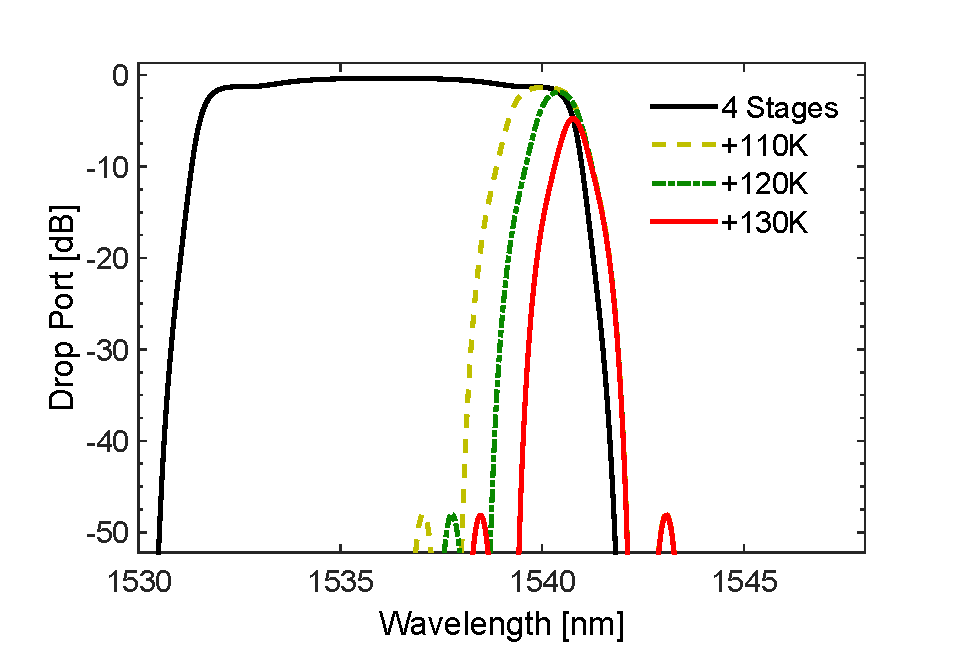
\includegraphics[width=.99\columnwidth]{data/4StageDesignCompiled2}
		\caption{Simulation of the spectral response with the heat applied to two out of four cascaded contra-DCs: the 1 dB bandwidth can be continuously tuned from 1007 GHz to  49GHz. The sidelobes stay under -49 dB even for small bandwidths due to the double filtering. This simulation doesn't consider fabrication phase noise.}
		\label{fig:bandTuneSimu}
	\end{figure} 
	
	For improved performance and flexibility, more stages can be cascaded.
	Fig.~\ref{fig:bandTuneSimu} shows our simulation results of a 4-stage cascade contra-DC filter, consisting of two pairs of identical contra-DCs with a stronger coupling than the one experimentally demonstrated (53.5~mm$^{-1}$ vs 38~mm$^{-1}$). Each pair is controlled by the same temperature, performing as a single tuning element.
	
	
	
	%\section{Conclusion}
	In summary, we have demonstrated a bandwidth tunable filter with a low insertion loss of less than~0.5 dB, low ripples of less than~0.3 dB, a large maximal bandwidth of greater than 750~GHz, and high contrast of 55~dB. 
	A large bandwidth tuning range over 670~GHz has been achieved, which, to the best of our knowledge, is the widest ever demonstrated on a silicon chip. 
	This ultra-wide bandwidth tunability makes the device very attractive for next-generation ultrahigh baud-rate applications (e.g., high-capacity super-channel transmissions) and flexible optical networking. 
	
	\section*{Acknowledgments}
	We acknowledge CMC Microsystems for the  software and the fabrication subsidy. We thank Yun Wang and Lukas Chrostowski with the University of British Columbia for the fiber grating coupler design. The authors acknowledge the Natural Sciences and Engineering Research Council of Canada for funding this research. This work is part of the SPEED research project (Silicon Photonic Electrically Engineered Devices) funded by NSERC (RDCPJ438811-12), PROMPT (PJT-2011-17), and TeraXion. The silicon chip was fabricated at the University of Washington Microfabrication/Nanotechnology User Facility, a member of the NSF National Nanotechnology Infrastructure Network.
	
	
	\bibliography{bibli}
	
\end{document}